\documentclass[../main.tex]{subfiles}

\begin{document}

\lstset{
	numbers=left,
	stepnumber=1,
	firstnumber=1,
	numberfirstline=true,
	xleftmargin=3em,
	xrightmargin=3em,
}

El proyecto se divide en varias fases: recopilación de artículos de investigación, lectura del contenido, preprocesado del contenido, extracción de información y presentación del resultado en XML.

En primer lugar se recopilan todas las muestras a tratar. Estas deben situarse en una misma carpeta.

Sigue una fase de lectura en la que se extrae el contenido utilizando las librerías \texttt{PyPDF2} (para metadatos) y \texttt{pdfminer.six} (para el contenido).

La siguiente fase es el preprocesado de la información. Aquí el proceso se divide, pues se prepara la información de distinta manera según sea para trabajar con los metadatos del PDF o su contenido.

Con los datos ya preparados se inicia la fase de extracción. Se usarán distintas técnicas según se trabaje con el texto plano o con los bloques de texto.

Por último, se exportan todos los metadatos a un XML. Estos siguen el estándar Dublin Core.

En las siguientes secciones se verán con detalle todas estas fases.

El flujo de información sigue el esquema de la figura \ref{fig:development-phases}.

\begin{figure}[h]
  \centering
    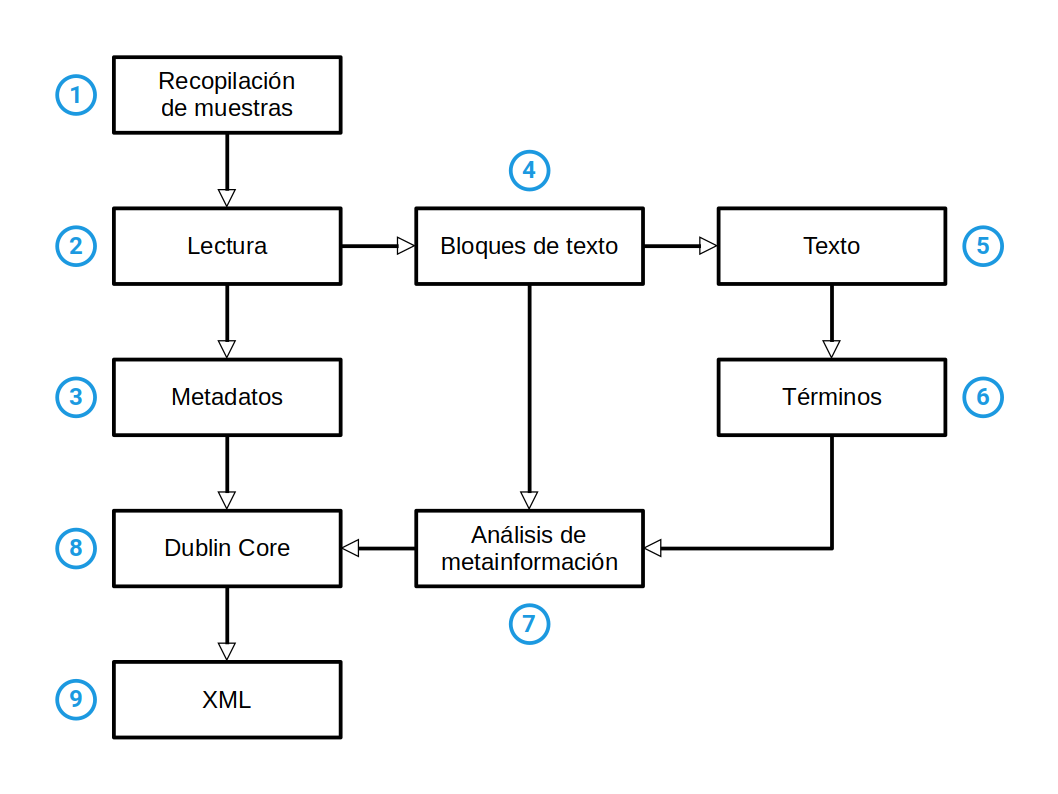
\includegraphics[width=0.7\textwidth]{../images/development-phases.png}
  \caption{Fases de desarrollo.}
  \label{fig:development-phases}
\end{figure}


\subsection{Recopilación}

Para realizar tanto las pruebas como para obtener unos resultados admisibles, se hizo una recopilación de artículos de investigación de PDF. En total se obtuvieron cien artículos de diferentes materias aunque de predominancia tecnológica.


\subsection{Lectura}

En primer lugar se leen los metadatos utilizando la librería \texttt{PyPDF2}. De este modo se consigue obtener una base de metainformación de la que partir.

Los metadatos necesitan un filtrado previo. Aquellos valores que estén vacíos o que solo contengan espacios en blanco, se eliminan.

Los campos de \texttt{DocumentInfo} se devuelven como cadena de texto. En el caso del autor se hace una separación de los nombres mediante expresiones regulares. Se parten teniendo en cuenta que la mayoría de los casos con varios autores estos están separados por comas o puntos y comas.

Los campos de \texttt{XmpMedatada} se devuelven con varios tipos según el campo. Se han reducido a tres casos:

\begin{itemize}
	\item cadenas de texto para los campos \texttt{coverage}, \texttt{format}, \texttt{idenfifier}, \texttt{source}
	\item listas de textos para los campos \texttt{contributor}, \texttt{creator}, description, \texttt{language}, \texttt{publisher}, \texttt{relation}, \texttt{rights}, \texttt{subject}, \texttt{title}, \texttt{type}
	\item lista de fechas para el campo date
\end{itemize}

El campo \texttt{dc:title} se transforma de diccionario a lista. Se da preferencia en el orden de la lista a los títulos en inglés o que sean por defecto. El resto de títulos, si son distintos, se añaden al final.

El campo \texttt{dc:creator} se le realiza una limpieza de cadenas vacías o que solo contengan espacios en blanco.

Después se lee el contenido. Esta fase se realiza en dos pasos.

Primeramente se lee todo el contenido como texto plano para un posterior procesamiento mediante NLP.

En segundo lugar se lee el contendido por bloques. Esta fase supone ya un preprocesado de información, que se utilizará posteriormente en la extracción de algunos metadatos como el título.

\subsection{Preprocesado}

La lectura del contenido de texto plano requiere un preprocesado antes de poder usarse. Este paso se realiza con la librería NLTK.

La lectura de bloques de texto ya realiza un preprocesado. Filtrando los bloques que no se necesitan, analizando la posición y el formato del texto y realizando algunos cálculos para su posterior uso.

La posición de los bloques de texto en el cuerpo del PDF se realiza mediante los margenes superior e izquierdo que separan al bloque del borde de la página. Estos márgenes se devuelven a modo de porcentaje, para evitar la influencia del tamaño de pagina a la hora de tener en cuenta los valores.

\subsection{Extracción}

La extracción de información se realiza mediante el análisis del contenido del documento. Dependiendo del metadato, el método empleado difiere de un caso a otro.

\textbf{Título}

Este metadato es el más identificativo de un documento. Independientemente que las palabras clave o el resumen puedan aportar una información más extensa del contenido, el título ofrece de un rápido vistazo una idea general del tema que se va a tratar en el artículo de investigación.

A diferencia de otros metadatos, este es más habitual que se encuentre definido en los metadatos del PDF. En la sección Resultados se 

Basándose en la revisión y análisis de los diferentes artículos, se observa que en la mayoría de ellos el título tiene una tipografía mayor que el resto. También se observa que la tipografía está en negrita, de forma que destaque de otros párrafos.

Además, si se tiene en cuenta la situación espacial del bloque de texto, se observa que los títulos se encuentran al inicio de la primera página.

Teniendo en cuenta todos estos factores se procede a realizar el procesamiento de los bloques de texto.

En primer lugar se recopilan todos los bloques de texto de la primera página. De todos estos bloques se calcula el máximo tamaño de letra.

Posteriormente, se filtran todos los bloques que tengan el tipo de letra igual al máximo obtenido.


Si el número de bloques es solo uno, se selecciona el texto del bloque. En otro caso, se realiza un segundo filtrado. Se seleccionan los bloques que tengan la tipografía en negrita. Al igual que en el caso anterior, si es uno, se selecciona el texto como resultado parcial.

\begin{lstlisting}[language=Python]
def __filter_text_blocks(self, text_blocks: list) -> list:
    max_font_size = self.__max_font_size(text_blocks)
    result_blocks = [b for b in text_blocks if b.font_size() == max_font_size
        and b.is_bold() and b.top_margin_percent < 50]
    if not result_blocks:
        result_blocks = [b for b in text_blocks if b.font_size() == max_font_size]
    return result_blocks
\end{lstlisting}

Si el número de bloques es mayor que uno, entonces se concatenan los textos bloques separados por un espacio.

Finalmente, y antes de devolver el resultado. Se realiza una limpieza de espacios en blanco y retornos de carro. El texto devuelto lo formará una solo línea de texto.

\textbf{Autor}

Los métodos probados para extraer el autor no dan resultados. Estos se encuentran en posiciones distintas, mezclados con otros datos (cargo, entidad, ciudad) y símbolos (referencias). Cuando se trata de aplicar el reconocimiento de entidades no se consigue establecer diferenciación entre los elementos. El factor de acierto no es el esperado.

\textbf{Descripción}

El campo descripción se extrae de los metadatos del PDF. Si este se encuentra vacío se procede al análisis del texto.

Para rellenar este metadato se utiliza el resumen (abstract) que poseen  los artículos de investigación. Este elemento se encuentra en la primera página, antes que cualquier otro contenido.

Para localizarlo se busca un bloque de texto que empiece por «abstract» y se almacena todo el párrafo que le sigue. En algunos casos, el título «abstract» se encuentra en un bloque que precede. Entonces se busca el bloque siguiente y se guarda.

Se dan casos que no se extrae el contenido correctamente. Cuando el resumen es muy extenso y ocupa más de una página. También cuando el resumen se encuentra dividido en secciones, que emplean cabeceras que se repiten en el resto del documento. Por ejemplo, un \textit{abstract} que contenga un apartado «Introduction» y unos párrafos después se encuentre una sección de igual nombre.

\textbf{Asunto}

El asunto, como ocurre en los demás casos, se extrae primeramente del XMP del PDF. Si este se encuentra vacío entonces se procede a analizar el texto. Hay dos opciones adicionales para su completado: expresiones regulares o términos más frecuentes.

En el primer caso, se emplea un método similar al que se utiliza con «description». Se busca en la primera página del documento un bloque que comience por el texto «keywords». El texto que le continúa hasta el final se consideran que son las palabras claves divididas por un separador. Se almacena entonces cada una de las palabras en una lista.

En el segundo caso, se emplea una técnica de procesamiento de lenguaje, que son los bigramas. Se trata de calcular la frecuencia de dos palabras seguidas a lo largo del texto. Se ha seleccionado bigramas en lugar de palabras más frecuentes porque aportan más información. Y bigramas en lugar de trigramas porque estas son menos frecuentes en el texto.

Utilizando estos tres métodos, se consigue que el campo «subject» nunca esté vacío.

\textbf{Idioma}

El idioma no es un campo de información especialmente útil para este estudio en concreto, dado que todos los artículos que se analizan deben estar en inglés.

Se ha incluido como medio de verificación, en caso de que se le proporcione un documento en otro idioma que no sea el inglés.

El valor que se toma por defecto es el que se incluye en el metadato del XMP del PDF. En caso de que se encontrara vacío, lo más habitual, se procede a detectar el idioma del contenido del documento.

Para identificarlo se utiliza la librería \texttt{langdetect}. Esta proporciona una interfaz bastante sencilla. Se le pasa un texto y devuelve el código ISO 639-1 del idioma con mayor probabilidad.

\begin{lstlisting}[language=Python]
def language(self) -> str:
    result = detect(self.text())
    if result != 'unknown':
        return result
    else:
        return ''
\end{lstlisting}

En caso de no haber una coincidencia positiva, devuelve el valor «unknown». Cuando esto suceda, no se rellenará el campo \texttt{language} en los metadatos Dublin Core.

\textbf{Número de páginas}

El cálculo del número de páginas se realiza directamente usando la librería \texttt{PyPdf2}. Esta separa el contenido del documento por páginas. El proceso es tan sencillo como calcular la longitud de dicha secuencia.

\begin{lstlisting}[language=Python]
    self.num_pages: int = len(reader.pages)
\end{lstlisting}

\textbf{Número de tablas}

Para contabilizar el número de tablas se hizo un primer intento con la librería \texttt{pdfminer.six} pero no se encontró ningún método que facilitar la identificación de una tabla en el cuerpo del PDF.

Posteriormente se investigó la posibilidad de emplear la librería tabula, pero está dedicada a extraer el contenido, no a su localización o contabilización.

Finalmente, se decide emplear expresiones regulares. Dado que las tablas deben llevar un pie identificativo, se localizan examinando el texto. Cualquier bloque texto que comience por la palabra «tabla» y se continúe por un número se considera que sucede a una tabla en el documento. Para evitar falsos positivos o tablas que se extiendan más de una página, se almacenan los números de tabla en un conjunto. Así se consigue que al contabilizar, se haga con identificadores de tabla únicos.

\textbf{Número de imágenes}

Otra de las estadísticas que se va a analizar es el número de figuras. En un primer intento se hizo un conteo de las imágenes del documento pero se vio que no cuadraban. Las razones son diversas, entre ellas: las figuras pueden componerse de varias imágenes, los artículos pueden tener una breve biografía de los autores con su fotografía, las cabeceras pueden incluir imágenes de la publicación, etc.

Aunque queda demostrado que no tiene utilidad para contabilizar las figuras, se ha mantenido esta estadística para su relación con el número de figuras.

Para realizar el conteo, se buscan las imágenes del documento y se anota su identificador. Este identificador no se especifica en la documentación de la librería \texttt{PyPDF2}. Se obtuvo la información de cómo se almacenan las imágenes revisando el código en el repositorio público.

Los identificadores de objeto no se encuentran en todas las imágenes. Cuando es nulo, se toma como identificador el nombre de la imagen.

Al finalizar la inspección del documento se cuentan todos los identificadores únicos, sin repeticiones, para obtener el número total de imágenes.

\textbf{Número de figuras}

El número de figuras se calcula de un modo similar al que se emplea para el número de tablas. Como ocurría en el caso anterior, no se consiguió mediante el uso de la librería \texttt{pdfminer.six}.

En el apartado anterior se describe el primer método empleado, que es contabilizando imágenes. Tras abandonar este método se decide emplear el mismo que las tablas, usando expresiones regulares.

Se trata de identificar un bloque de texto que comience por el texto «figura» o simplemente su abreviatura «fig». Luego se busca el número identificativo que le sigue y se anota para descartar los valores repetidos. Al finalizar la lectura de todo el documento se obtiene una lista de valores únicos de figuras.

\subsection{Presentación}

La salida de datos se realiza en XML. Para las etiquetas de los metadatos se sigue el estándar Dublin Core. Aparte se añaden algunas propiedades personalizadas para los metadatos de conteo: número de páginas, de tablas y de figuras. Estos se incluyen en forma de atributos, junto con el nombre del fichero.

\subsection{Pruebas}

Se han realizado una serie de pruebas de las clases creadas.
Como caso ilustrativo se mostrará el del metadato título de la clase \texttt{PdfReader}.

\begin{lstlisting}[language=Python]
	def test_abstract(self):
	    for item in self.pa:
	        self.assertEqual(item['reader'].abstract(), item['tsv']['description'])
	
	def test_figure_count(self):
	    for item in self.pa:
	        self.assertEqual(item['reader'].figure_count, int(item['tsv']['figures']))
	
	def test_keywords(self):
	    for item in self.pa:
	        subject = item['tsv']['subject'].split(' ; ') if item['tsv']['subject'] else []
	    self.assertEqual(item['reader'].keywords(), subject)
	
	def test_table_count(self):
	    for item in self.pa:
	        self.assertEqual(item['reader'].table_count, int(item['tsv']['tables']))
	
	def test_title(self):
	    for item in self.pa:
	        self.assertEqual(item['reader'].title(), item['tsv']['title'])
\end{lstlisting}

\begin{figure}[h]
	\centering
	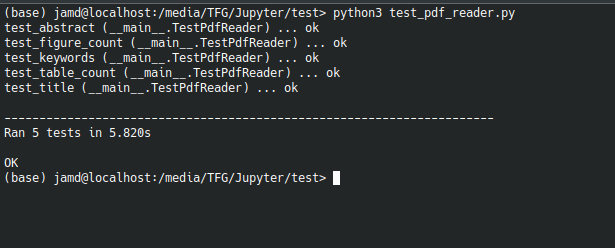
\includegraphics[width=0.9\linewidth]{../images/test-pdf-reader}
	\caption{Resultados del test de la clase PdfReader}
	\label{fig:test-pdf-reader}
\end{figure}

\end{document}
